\tikzset{every picture/.style={line width=0.75pt}} %set default line width to 0.75pt        

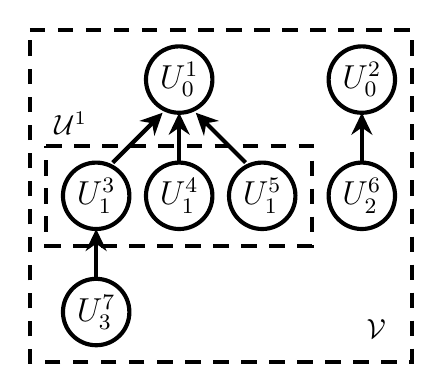
\begin{tikzpicture}[x=0.6pt,y=0.6pt,yscale=-1,xscale=1]
	%uncomment if require: \path (0,300); %set diagram left start at 0, and has height of 300
	
	%Shape: Circle [id:dp821654118938725] 
	\draw  [line width=1.5]  (130,70) .. controls (130,58.95) and (138.95,50) .. (150,50) .. controls (161.05,50) and (170,58.95) .. (170,70) .. controls (170,81.05) and (161.05,90) .. (150,90) .. controls (138.95,90) and (130,81.05) .. (130,70) -- cycle ;
	%Shape: Circle [id:dp7532382575897598] 
	\draw  [line width=1.5]  (80,140) .. controls (80,128.95) and (88.95,120) .. (100,120) .. controls (111.05,120) and (120,128.95) .. (120,140) .. controls (120,151.05) and (111.05,160) .. (100,160) .. controls (88.95,160) and (80,151.05) .. (80,140) -- cycle ;
	%Shape: Circle [id:dp5902978501813476] 
	\draw  [line width=1.5]  (180,140) .. controls (180,128.95) and (188.95,120) .. (200,120) .. controls (211.05,120) and (220,128.95) .. (220,140) .. controls (220,151.05) and (211.05,160) .. (200,160) .. controls (188.95,160) and (180,151.05) .. (180,140) -- cycle ;
	%Straight Lines [id:da9016881764549007] 
	\draw [line width=1.5]    (137.17,92.83) -- (110,120) ;
	\draw [shift={(140,90)}, rotate = 135] [fill={rgb, 255:red, 0; green, 0; blue, 0 }  ][line width=0.08]  [draw opacity=0] (13.4,-6.43) -- (0,0) -- (13.4,6.44) -- (8.9,0) -- cycle    ;
	%Straight Lines [id:da026586992089503658] 
	\draw [line width=1.5]    (162.83,92.83) -- (190,120) ;
	\draw [shift={(160,90)}, rotate = 45] [fill={rgb, 255:red, 0; green, 0; blue, 0 }  ][line width=0.08]  [draw opacity=0] (13.4,-6.43) -- (0,0) -- (13.4,6.44) -- (8.9,0) -- cycle    ;
	%Straight Lines [id:da8305170432215097] 
	\draw [line width=1.5]    (150,94) -- (150,120) ;
	\draw [shift={(150,90)}, rotate = 90] [fill={rgb, 255:red, 0; green, 0; blue, 0 }  ][line width=0.08]  [draw opacity=0] (13.4,-6.43) -- (0,0) -- (13.4,6.44) -- (8.9,0) -- cycle    ;
	%Shape: Circle [id:dp5384623722514443] 
	\draw  [line width=1.5]  (130,140) .. controls (130,128.95) and (138.95,120) .. (150,120) .. controls (161.05,120) and (170,128.95) .. (170,140) .. controls (170,151.05) and (161.05,160) .. (150,160) .. controls (138.95,160) and (130,151.05) .. (130,140) -- cycle ;
	%Shape: Circle [id:dp16437012307038867] 
	\draw  [line width=1.5]  (80,210) .. controls (80,198.95) and (88.95,190) .. (100,190) .. controls (111.05,190) and (120,198.95) .. (120,210) .. controls (120,221.05) and (111.05,230) .. (100,230) .. controls (88.95,230) and (80,221.05) .. (80,210) -- cycle ;
	%Shape: Circle [id:dp734554865123197] 
	\draw  [line width=1.5]  (240,70) .. controls (240,58.95) and (248.95,50) .. (260,50) .. controls (271.05,50) and (280,58.95) .. (280,70) .. controls (280,81.05) and (271.05,90) .. (260,90) .. controls (248.95,90) and (240,81.05) .. (240,70) -- cycle ;
	%Shape: Circle [id:dp48143471465976706] 
	\draw  [line width=1.5]  (240,140) .. controls (240,128.95) and (248.95,120) .. (260,120) .. controls (271.05,120) and (280,128.95) .. (280,140) .. controls (280,151.05) and (271.05,160) .. (260,160) .. controls (248.95,160) and (240,151.05) .. (240,140) -- cycle ;
	%Straight Lines [id:da6721182832003427] 
	\draw [line width=1.5]    (100,164) -- (100,171) -- (100,190) ;
	\draw [shift={(100,160)}, rotate = 90] [fill={rgb, 255:red, 0; green, 0; blue, 0 }  ][line width=0.08]  [draw opacity=0] (13.4,-6.43) -- (0,0) -- (13.4,6.44) -- (8.9,0) -- cycle    ;
	%Straight Lines [id:da34999125713295975] 
	\draw [line width=1.5]    (260,94) -- (260,120) ;
	\draw [shift={(260,90)}, rotate = 90] [fill={rgb, 255:red, 0; green, 0; blue, 0 }  ][line width=0.08]  [draw opacity=0] (13.4,-6.43) -- (0,0) -- (13.4,6.44) -- (8.9,0) -- cycle    ;
	%Shape: Rectangle [id:dp18541931062860906] 
	\draw  [dash pattern={on 5.63pt off 4.5pt}][line width=1.5]  (60,40) -- (290,40) -- (290,240) -- (60,240) -- cycle ;
	%Shape: Rectangle [id:dp6446344359743517] 
	\draw  [dash pattern={on 5.63pt off 4.5pt}][line width=1.5]  (70,110) -- (230,110) -- (230,170) -- (70,170) -- cycle ;
	
	% Text Node
	\draw (150,70) node  [font=\large]  {$U_{0}^{1}$};
	% Text Node
	\draw (100,140) node  [font=\large]  {$U_{1}^{3}$};
	% Text Node
	\draw (200,140) node  [font=\large]  {$U_{1}^{5}$};
	% Text Node
	\draw (150,140) node  [font=\large]  {$U_{1}^{4}$};
	% Text Node
	\draw (100,210) node  [font=\large]  {$U_{3}^{7}$};
	% Text Node
	\draw (260,70) node  [font=\large]  {$U_{0}^{2}$};
	% Text Node
	\draw (260,140) node  [font=\large]  {$U_{2}^{6}$};
	% Text Node
	\draw (73,87.4) node [anchor=north west][inner sep=0.75pt]    {$\mathcal{U}^{1}$};
	% Text Node
	\draw (261,212.4) node [anchor=north west][inner sep=0.75pt]    {$\mathcal{V}$};
	
	
\end{tikzpicture}
